\subsection{Теорема о непрерывном D-оптимальном плане}
Модель наблюдений:
\begin{gather} \label{model:start}
y_i = \theta_0 + \theta_1 x_{i1} + \theta_2 x_{i2} + \varepsilon(x^{(i)}), i = \overline{1, n}, n \ge 3 \\
E\{ \varepsilon(x^{(i)}) \} = 0, E\{ \varepsilon^{(i)}\ \varepsilon^{(j)} \} = 0, i \ne j \\
D\{ \varepsilon(x^{(i)}) \} = d(x_{i1}, x_{i2}) > 0, \\
d(x_1, x_2) \ge \frac{\sigma^2}{3}(1 + x_1^2 + x_2^2) \label{model:end}
\end{gather}
$$ -1 \le x_{ij} \le 1, j = \overline{1, 2}, i = \overline{1, n}$$
Для дисперсии наблюдений $d(x_1, x_2)$ предполагается, что:
\begin{equation}\label{model:dispersion}
d(x_1, x_2) \ge \frac{\sigma^2}{3}(1 + x_1^2 + x_2^2), \sigma > 0.
\end{equation}

Причем \eqref{model:dispersion} обращается в равенство в вершинах спектра плана:
\begin{equation}\label{plan-points}
\begin{gathered}
x^{(1)}=(1, 1); \\
x^{(2)}=(-1, 1); \\
x^{(3)}=(-1, -1); \\
x^{(4)}=(1, -1)
\end{gathered}
\end{equation}
Введём обозначния: $d(x^{(1)}) = d_1, d(x^{(2)}) = d_2, d(x^{(3)}) = d_3, d(x^{(4)}) = d_4$

\begin{theorem}\label{main-theorem}[о непрерывном D-оптимальном плане в точках спектрах плана]
	Для модели наблюдений \eqref{model:start}-\eqref{model:end} с не коррелированными ошибками наблюдений, имеющими средние значения ноль и дисперсии $d(x_1, x_2)$, следующие планы являются непрерывными $D$-оптимальными. План
	\begin{equation} \label{main-theorem:plan-1}
	\varepsilon_1^{0} = \left \{ 
	\underset{\frac 1 3} {x^{(1)}},
	\underset{\frac 1 3} {x^{(2)}},
	\underset{\frac 1 3} {x^{(3)}}
	\right \}
	\end{equation}
	с дисперисиями наблюдений
	\begin{equation}
	d(x_1, x_2) \ge \frac 1 4 (d_1 + d_3 + 2 d_1 x_1 - 2 d_3 x_2 - 2d_2 x_1 x_2 + (d_1 + d_2)x_1^2 + (d_2 + d_3)x_2^2).
	\end{equation}
	
	План
	\begin{equation}
	\varepsilon_2^{0} = \left \{ 
	\underset{\frac 1 3} {x^{(2)}},
	\underset{\frac 1 3} {x^{(3)}},
	\underset{\frac 1 3} {x^{(4)}}
	\right \}
	\end{equation}
	с дисперисиями наблюдений
	\begin{equation}
	d(x_1, x_2) \ge \frac 1 4 (d_2 + d_4 + 2 d_4 x_1 + 2 d_2 x_2 + 2 d_3 x_1 x_2 + (d_3 + d_4)x_1^2 + (d_2 + d_3)x_2^2).
	\end{equation}
	
	План
	\begin{equation}
	\varepsilon_3^{0} = \left \{ 
	\underset{\frac 1 3} {x^{(1)}},
	\underset{\frac 1 3} {x^{(3)}},
	\underset{\frac 1 3} {x^{(4)}}
	\right \}
	\end{equation}
	с дисперисиями наблюдений
	\begin{equation}
	d(x_1, x_2) \ge \frac 1 4 (d_1 + d_3 - 2 d_3 x_1 + 2 d_1 x_2 - 2 d_4 x_1 x_2 + (d_3 + d_4)x_1^2 + (d_1 + d_4)x_2^2).
	\end{equation}
	
	План
	\begin{equation}
	\varepsilon_4^{0} = \left \{ 
	\underset{\frac 1 3} {x^{(1)}},
	\underset{\frac 1 3} {x^{(2)}},
	\underset{\frac 1 3} {x^{(4)}}
	\right \}
	\end{equation}
	с дисперисиями наблюдений
	\begin{equation}
	d(x_1, x_2) \ge \frac 1 4 (d_2 + d_4 - 2 d_2 x_1 - 2 d_4 x_2 + 2 d_1 x_1 x_2 + (d_1 + d_2)x_1^2 + (d_1 + d_4)x_2^2).
	\end{equation}
	(\ref{main-theorem}) описывает непрерывный D-оптимальный план для модели (6)-(8) в точках $x^{(3)}, x^{(4)}, x^{(1)}$.\\
\end{theorem}
\textbf{Доказательство}.
Опишем вначале процесс построения непрерывного D-оптимального плана $\varepsilon_3^0$.
Для оптимального плана  $\varepsilon_1^{0}$, по теореме эквивалентности Кифера - Вольфовица [5], выполняется неравенство:
\begin{equation}\label{main-theorem:ineq}
\frac 1 {d(x_1, x_2)}
(1, x_1, x_2)
M^{-1}(\varepsilon_1^0)
\begin{pmatrix}1 \\ x_1 \\ x_2 \end{pmatrix} \le 3,
|x_1| \le 1, |x_2| \le 1,
\end{equation}
где $d(x_1, x_2)$ - непрерывная функция, определяющая дисперсию ошибки наблюдения в точке (x1, x2), $M(\varepsilon_1^{0})$ - информационная матрица плана экспериментов. В точках спектра плана $\varepsilon_1^{0}$ неравенство \eqref{main-theorem:ineq}, как необходимое условие, обращается в равенство. Исходя из этих условий, построим класс функций $d(x_1, x_2)$, определяющих поведение дисперсии ошибок наблюдений  для плана $\varepsilon_1^{0}$. Информационная матрица плана $\varepsilon_1^{0}$ равна:
\begin{gather*}
M(\varepsilon_1^0) = \frac 1 3 \left(
\frac 1 d_1 \begin{pmatrix} 1 \\ 1 \\ 1 \end{pmatrix} (1, 1, 1) + 
\frac 1 d_2 \begin{pmatrix} 1 \\ -1 \\ 1 \end{pmatrix} (1, -1, 1) + 
\frac 1 d_3 \begin{pmatrix} 1 \\ -1 \\ -1 \end{pmatrix} (1, -1, -1)
\right) \\ =
\frac 1 3 
\begin{pmatrix}
a & b & c \\
b & a & e \\
c & e & a
\end{pmatrix},
\end{gather*}
где
\begin{equation}\label{main-theorem:defs} \begin{split}
a=d_1^{-1}+d_2^{-1}+d_3^{-1},\\
b=d_1^{-1}-d_2^{-1}-d_3^{-1},\\
c=d_1^{-1}+d_2^{-1}-d_3^{-1},\\
d=d_1^{-1}-d_2^{-1}+d_3^{-1}.
\end{split}\end{equation}
Тогда обратная к матрице $M(\varepsilon_1^0)$ имеет вид:
\begin{equation} \label{main-theorem:inv-matrix}
M^{-1}(\varepsilon_1^0) = \frac 3 {a^3 + 2 b c e - a(b^2 + c^2 + e^2)}
\begin{pmatrix}
a^2 - e^2,& ce - ab, & be - ac\\
ce - ab,& a^2-c^2,& bc-ae\\
be - ac,& bc - ae,& a^2 - b^2			
\end{pmatrix} 
\end{equation}.
Разрешая неравенство \eqref{main-theorem:ineq} относительно $d(x_1, x_2)$ с учетом \eqref{main-theorem:inv-matrix} получим класс функций $d(x_1, x_2)$, определяющих изменение
дисперсии наблюдений в плане $\varepsilon_1^0$:
\begin{equation} \label{main-theorem:d-f-ineq}
d(x_1, x_2) \ge f(x_1, x_2)
\end{equation}
где
\begin{multline}
f(x_1, x_2) =
\frac {1}{a^3 + 2bce - a(b^2+c^2+e^2)} \times \\
\times [{a^2 - e^2 +2(ce - ab)x_1 + 2(be-ac)x_2 + 2(bc - ae)x_1 x_2 + (a^2 - c^2)x_1^2 + (a^2 - b^2)x_2^2}].		
\end{multline}
Если теперь в функции $f(x_1, x_2)$ вернуться к исходным обозначениям \eqref{main-theorem:defs}, то неравенство \eqref{main-theorem:d-f-ineq} обратится в неравенство \eqref{main-theorem:plan-1}. Необходимое условие оптимальности плана также выполняется, так как в точках спектра плана $x^{(1)}, x^{(2)}, x^{(3)}$  неравенство \eqref{main-theorem:plan-1} обращается в равенство.

Справедливость теоремы для планов $\varepsilon_2^0, \varepsilon_3^0,\varepsilon_4^0$ доказывается аналогично, однако меняются обозначения \eqref{main-theorem:defs}.\\ Для $\varepsilon_2^0$:
\begin{equation*} \begin{split}
a=d_2^{-1}+d_3^{-1}+d_4^{-1},\\
b=-d_2^{-1}-d_3^{-1}+d_4^{-1},\\
c=d_2^{-1}-d_3^{-1}-d_4^{-1},\\
d=-d_2^{-1}+d_3^{-1}-d_4^{-1};
\end{split}\end{equation*}
для $\varepsilon_3^0$:
\begin{equation*} \begin{split}
a=d_1^{-1}+d_3^{-1}+d_4^{-1},\\
b=d_1^{-1}-d_3^{-1}+d_4^{-1},\\
c=d_1^{-1}-d_3^{-1}-d_4^{-1},\\
d=d_1^{-1}+d_3^{-1}-d_4^{-1};
\end{split}\end{equation*}
для $\varepsilon_4^0$:
\begin{equation*} \begin{split}
a=d_1^{-1}+d_2^{-1}+d_4^{-1},\\
b=d_1^{-1}-d_2^{-1}+d_4^{-1},\\
c=d_1^{-1}+d_2^{-1}-d_4^{-1},\\
d=d_1^{-1}-d_2^{-1}-d_3^{-1};
\end{split}\end{equation*}
\textbf{Теорема доказана}.


\subsection{Пример применения теоремы}
Рассмотрим план в точках $x^{(3)}, x^{(4)}, x^{(1)}$.\\
Пусть $d(x_1, x_2)$ такая, что в указанных точках проходит через поверхность $z = 4 + x_1 + x_2$.
Тогда
\begin{gather*}
d_1 = d(x_1^{(1)}, x_2^{(1)}) = 4 + 1 + 1 = 6 \\
d_2 = d(x_1^{(2)}, x_2^{(2)}) = 4 -1 + 1 = 4 \\
d_3 = d(x_1^{(3)}, x_2^{(3)}) = 4 -1 - 1 = 2 \\
d_4 = d(x_1^{(4)}, x_2^{(4)}) = 4 + 1 - 1 = 4
\end{gather*}
Используя доказанную теорему, можно получить, что
$$d(x_1, x_2) \ge 2 - x_1 + 3x_2 -2x_1x_2 +\frac{3}{2}x_1^2 + \frac 5 2 x_2^2.$$
Канонический вид поверхности (эллиптический параболоид):\\
$$x^2 (4 - \sqrt{5}) + y^2 (4 + \sqrt 5) = 2z$$
График поверхности:\\
\begin{center}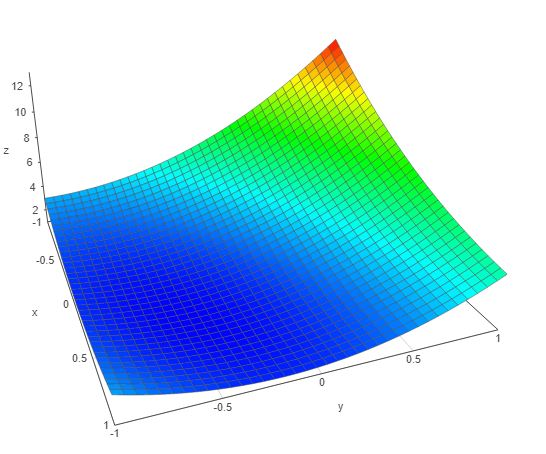
\includegraphics[scale=0.5]{plot134.jpg}\end{center}

Используя аналогичные рассуждения, для остальных планов можно получить:
\begin{enumerate}
	\item Для плана в точках $x^{(1)}, x^{(2)}, x^{(3)}$:
	$$d(x_1, x_2) \ge 2 + 3x_1 - x_2 -2x_1x_2 +\frac{5}{2}x_1^2 + \frac 3 2 x_2^2.$$
	Канонический вид поверхности:
	$$x^2 (4 - \sqrt{5}) + y^2 (4 + \sqrt 5) = 2z$$
	График поверхности:\\
	\begin{center}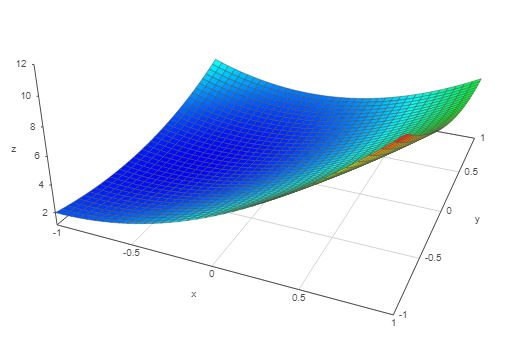
\includegraphics[scale=0.5]{plot123.jpg}\end{center}
	
	\item План в точках $x^{(1)}, x^{(2)}, x^{(4)}$:
	$$d(x_1, x_2) \ge 2 - 2x_1 - 2x_2 +3x_1x_2 +\frac{5}{2}x_1^2 + \frac 5 2 x_2^2$$
	Канонический вид поверхности:
	$$x^2 + 4y^2 = z$$
	График поверхности:\\
	\begin{center}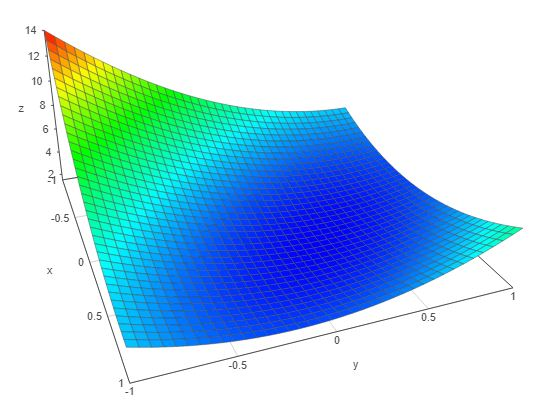
\includegraphics[scale=0.5]{plot124.jpg}\end{center}
	\item План в точках $x^{(2)}, x^{(3)}, x^{4)}$:
	$$d(x_1, x_2) \ge 2 + 2x_1 + 2x_2 +x_1x_2 +\frac{3}{2}x_1^2 + \frac 3 2 x_2^2$$
	Канонический вид поверхности:
	$$x^2 + 2 y^2 = z$$
	График поверхности:\\
	\begin{center}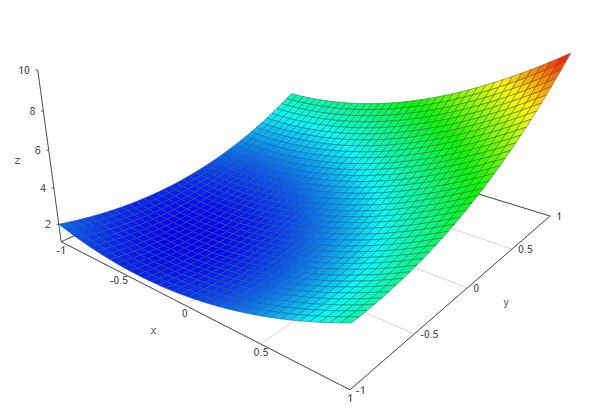
\includegraphics[scale=0.5]{plot234.jpg}\end{center}
\end{enumerate}

\subsection{Программная проверка оптимальности}
Подтвердим полученные результаты практически. Для этого была написана программа, которая перебирает все возможные планы исходной задачи и находит оптимальный.\\
Программа написана на языке Python с использованием пакетов numpy, scipy.\\
Приведем ее исходный код:
\lstinputlisting[language=Python,tabsize=2]{listings/check_optimal_in_points.py}

Вывод программы:
\lstinputlisting[numbers=none]{listings/check_optimal_in_points_output.txt}
Результат работы программы подтверждает теоретические рассуждения.


\subsection {Символьная проверка оптимальности}
В предыдущем параграфе оптимальность построенных планов была показана численно для заданной функции дисперсии. Покажем символьно, что неравенство \eqref{main-theorem:ineq} действительно обращается в равенство в вершинах спектра плана.\\
Для доказательства этого факта была написана программа в среде Matlab.
Указанная программа проверяет, что построенные планы в вершинах спектра плана в точности обращаются в значение дисперсии в заданной точке.
Приведём её листинг:
\lstinputlisting[language=Matlab,tabsize=2]{listings/symbol_check_optimality.txt}

Результат работы программы:
\lstinputlisting[numbers=none]{listings/symbol_check_optimality_output.txt}

Видно, что равенства выполняются.